\chapter{Reference manual of infoDecompuTE package} \label{append:infoDecompuTE}

\includepdf[pages={1-},scale=1]{ChapterAppendix/infoDecompuTE.pdf}

\chapter{The Information matrix in more detail} \label{append:informatSym}
This Chapter is to show that the information matrix $\Z' (\I-\mP_{r})(\I -\mP_{\gamma}) \Z$ used for the objective function is symmetric. 

Let $\mP_r$ and $\mP_\gamma$ be orthogonal projection matrices, then 
\[
\mP_r = \mP_r^2 = \mP_r\mP_r \; \; \mathrm{and} \; \; \mP_r = \mP_r'
\]
So 
\begin{eqnarray}
\nonumber &&	\Z' (\I-\mP_{r})(\I -\mP_{\gamma}) \Z\\
\nonumber &=& 	\Z' (\I-\mP_{r} - \mP_{\gamma} + \mP_{r}\mP_{\gamma}) \Z\\
\nonumber &=&	\Z' \Z - \Z'\mP_{r} \Z  - \Z' \mP_{\gamma}\Z  + 2\Z' \mP_{r}\mP_{\gamma}\Z\\
\label{eq:informatSym} &=&	\Z' \Z - (\mP_{r}\Z)'\Z\mP_{r} - (\mP_{\gamma}\Z )'\mP_{\gamma}\Z  + 2\Z' \mP_{r}\mP_{\gamma}\Z\\
\end{eqnarray}
where $\Z' \Z$, $(\mP_{r}\Z)'\Z\mP_{r}$ and $(\mP_{\gamma}\Z )'\mP_{\gamma}\Z$ are symmetric. 

The projection matrix which projects $\bm{y}$ onto the Between Runs vector subspace is 
\[
\mP_{r} = \W_{r}(\W_{r}'\W_{r})^{-1} \W_{r}'
\]
where $\W_{r}$ is design matrix for Run factor of the Phase 2 experiment and can be expressed as 
\[
 \W_{r} = \mathbf{1}_{n_\gamma} \otimes \I{n_r}.
\]
Thus, projection matrix for Between Runs can be re-written as  
\[
\mP_{r} =\frac{1}{n_\gamma} \mathbf{1}_{n_\gamma}  \mathbf{1}_{n_\gamma}' \otimes \I{n_r}.
\]

The projection matrix which projects $\bm{y}$ onto the Between Tags vector subspace is 
\[
\mP_{\gamma} = \X_{\gamma}(\X_{\gamma}'\X_{\gamma})^{-1}\X_{\gamma}
\]
where $\X_{\gamma}$ is design matrix for Tag factor of the Phase 2 experiment and can be expressed as 
\[
\X_{\gamma} = \I{n_\gamma} \otimes \mathbf{1}_{n_r} 
\]
Thus, projection matrix for Between Tags can be re-written as  
\[
\mP_{\gamma} = \frac{1}{n_r} \I{n_\gamma} \otimes \mathbf{1}_{n_r}\mathbf{1}_{n_r}'.
\]

This follow by $\mP_{r}\mP_{\gamma}$ in \ref{eq:informatSym} becomes 
\begin{eqnarray}
\nonumber \mP_{r}\mP_{\gamma}  &=& \frac{1}{n_r n_\gamma}  \mathbf{1}_{n_\gamma}  \mathbf{1}_{n_\gamma}' \otimes \mathbf{1}_{n_r}\mathbf{1}_{n_r}'\\
\nonumber &=& \frac{1}{n}  \mathbf{1}_{n_\gamma n_r}  \mathbf{1}_{n_\gamma n_r}' \\
\nonumber &=& \frac{1}{n}  \mathbf{1}_{n}  \mathbf{1}_{n}' \\
\nonumber &=&	\K_{n}. \\
\end{eqnarray}
Thus,  $\mP_{r}\mP_{\gamma} = \K$, then
\[ \Z' \mP_{r}\mP_{\gamma}\Z =  \frac{1}{n} \Z' \mathbf{1} \mathbf{1}' \Z  = \frac{1}{n} (\Z' \mathbf{1}) (\Z' \mathbf{1})'. \] 

Let
\[Z = 
\begin{pmatrix}  
a_{11} & a_{12} & a_{13} \\
a_{21} & a_{22} & a_{23} \\             
a_{31} & a_{32} & a_{33} \\
\end{pmatrix},
\]
then
\[ Z' \mathbf{1} = 
\begin{pmatrix}  
a_{.1} \\
a_{.2}\\             
a_{.3}  \\
\end{pmatrix}.
\]
So, 
\begin{eqnarray}
\nonumber (\Z' \mathbf{1}) (\Z' \mathbf{1})' 
\nonumber &=& \begin{pmatrix}  
a_{.1} \\
a_{.2}\\             
a_{.3}  \\
\end{pmatrix}
 \begin{pmatrix}  
a_{.1} & a_{.2} & a_{.3}\\
\end{pmatrix} \\
\nonumber &=&\begin{pmatrix}  
a_{.1}^2 & a_{.1}a_{.2} & a_{.1}a_{.3} \\
a_{.2}a_{.1} & a_{.2}^2 & a_{.2}a_{.3} \\             
a_{.3}a_{.1} & a_{.3}a_{.2} & a_{.3}^2 \\
\end{pmatrix}. 
\end{eqnarray}
Thus, $\Z' \mP_{r}\mP_{\gamma}\Z$ is also symmetric.  

\chapter{Various matrices from the example in Section~\ref{sec:theorANOVAtab}} \label{append:theorANOVAtab}

The orthogonal projection matrix of Within Runs and Tags vector subspace is given by
\[
\Q_{r\gamma} = 
\begin{bmatrix} 
 0.38 & -0.12 & -0.12 & -0.12 & -0.38 & 0.12 & 0.12 & 0.12 \\ 
  -0.12 & 0.38 & -0.12 & -0.12 & 0.12 & -0.38 & 0.12 & 0.12 \\ 
  -0.12 & -0.12 & 0.38 & -0.12 & 0.12 & 0.12 & -0.38 & 0.12 \\ 
  -0.12 & -0.12 & -0.12 & 0.38 & 0.12 & 0.12 & 0.12 & -0.38 \\ 
  -0.38 & 0.12 & 0.12 & 0.12 & 0.38 & -0.12 & -0.12 & -0.12 \\ 
  0.12 & -0.38 & 0.12 & 0.12 & -0.12 & 0.38 & -0.12 & -0.12 \\ 
  0.12 & 0.12 & -0.38 & 0.12 & -0.12 & -0.12 & 0.38 & -0.12 \\ 
  0.12 & 0.12 & 0.12 & -0.38 & -0.12 & -0.12 & -0.12 & 0.38 \\ 
\end{bmatrix} . 
\]

The animal information matrix in the Within Runs and Tags vector subspace is given by 
\[
\A_{a} = 
 \Z_{a}' Q_{r\gamma} \Z_{a} = 
\begin{bmatrix} 
 1 & -1 & 0 & 0 \\ 
 -1 & 1 & 0 & 0 \\ 
 0 & 0 & 1 & -1 \\ 
 0 & 0 & -1 & 1 \\ 
\end{bmatrix}.  
\]


The treatment information matrix of animals in the Within Runs and Tags vector subspace is given by 
\[
\A_{\tau} = 
 \X_{a}' Q_{r\gamma} \X_{a} = 
\begin{bmatrix} 
 2 & -2 \\ 
 -2 & 2 \\ 
\end{bmatrix}.  
\]

\chapter{Various matrices from the example in Subsection~\ref{sub:compareMSvsA}} \label{append:compareMSvsA}


The animal information matrix in the Within Runs and Tags vector subspace of the MS-optimal design is given by 
\[
\A_{a} = 
 \Z_{a}' \Q_{r\gamma} \Z_{a} = 
\begin{bmatrix} 
 1.17 & -0.25 & -0.25 & -0.25 & -0.17 & -0.25 \\ 
 -0.25 & 1.17 & -0.25 & 0.08 & -0.25 & -0.50 \\ 
 -0.25 & -0.25 & 1.17 & -0.50 & -0.25 & 0.08 \\ 
 -0.25 & 0.08 & -0.50 & 1.17 & -0.25 & -0.25 \\ 
 -0.17 & -0.25 & -0.25 & -0.25 & 1.17 & -0.25 \\ 
 -0.25 & -0.50 & 0.08 & -0.25 & -0.25 & 1.17 \\ 
\end{bmatrix}.  
\]


The animal information matrix in the Within Runs and Tags vector subspace of the A-optimal design is given by 
\[
\A_{a} = 
 \Z_{a}' \Q_{r\gamma} \Z_{a} = 
\begin{bmatrix} 
  1.17 & -0.83 & 0.33 & -0.17 & -0.17 & -0.33 \\ 
 -0.83 & 1.17 & 0.33 & -0.17 & -0.17 & -0.33 \\ 
 0.33 & 0.33 & 0.67 & -0.33 & -0.33 & -0.67 \\ 
 -0.17 & -0.17 & -0.33 & 1.17 & -0.83 & 0.33 \\ 
 -0.17 & -0.17 & -0.33 & -0.83 & 1.17 & 0.33 \\ 
 -0.33 & -0.33 & -0.67 & 0.33 & 0.33 & 0.67 \\ 
\end{bmatrix}.  
\]


\chapter{Various matrices from the example in Subsection~\ref{sub:maxTrtInfo}} \label{append:maxTrtInfo}
The animal information matrix in the Within Runs and Tags vector subspace of the optimal design obtained from the objective function with equal weights is given by 
\[
\A_{a} = 
 \Z_{a}' \Q_{r\gamma} \Z_{a} = 
\begin{bmatrix} 
 2.00 & -0.67 & -0.67 & -0.67 \\ 
 -0.67 & 2.00 & -0.67 & -0.67 \\ 
 -0.67 & -0.67 & 2.00 & -0.67 \\ 
 -0.67 & -0.67 & -0.67 & 2.00 \\ 
\end{bmatrix}.  
\]


The treatment information matrix of animals in the Within Runs and Tags vector subspace of the optimal design obtained from the objective function with equal weights is given by 
\[
\A_{\tau} = 
 \X_{a}' Q_{r\gamma} \X_{a} = 
\begin{bmatrix} 
2.67 & -2.67 \\ 
-2.67 & 2.67 \\ 
\end{bmatrix}.  
\]


The animal information matrix in the Within Runs and Tags vector subspace of the optimal design obtained from the objective function with greater weight on $E_a$ is given by 
\[
\A_{a} = 
 \Z_{a}' \Q_{r\gamma} \Z_{a} = 
\begin{bmatrix} 
 2.00 & -1.00 & -1.00 & -0.00 \\ 
  -1.00 & 2.00 & -1.00 & -0.00 \\ 
  -1.00 & -1.00 & 2.00 & -0.00 \\ 
  -0.00 & -0.00 & -0.00 & 0.00 \\ 
\end{bmatrix}.  
\]

The treatment information matrix of animals in the Within Runs and Tags vector subspace of the optimal design obtained from the objective function with greater weight on $E_a$ is given by 
\[
\A_{\tau} = 
 \X_{a}' Q_{r\gamma} \X_{a} = 
\begin{bmatrix} 
 2 & -2 \\ 
 -2 & 2 \\ 
\end{bmatrix}.  
\]

\chapter{Various matrices from the example in Section~\ref{sub:trtDF}} \label{append:trtDF}
The treatment information matrix of animals in the Within Runs and Tags vector subspace of the optimal design obtained from the objective function without maximising the treatment DF is given by 
\[
\A_{\tau} = 
 \X_{a}' Q_{r\gamma} \X_{a} = 
\begin{bmatrix} 
  2.00 & -2.00 & -0.00 \\ 
  -2.00 & 2.00 & -0.00 \\ 
  -0.00 & -0.00 & -0.00 \\ 
\end{bmatrix}.  
\]

The treatment information matrix of animals in the Within Runs and Tags vector subspace of the optimal design obtained from the objective function with maximising the treatment DF is given by 
\[
\A_{\tau} = 
 \X_{a}' Q_{r\gamma} \X_{a} = 
\begin{bmatrix} 
  2.50 & -1.00 & -1.50 \\ 
  -1.00 & 2.00 & -1.00 \\ 
  -1.50 & -1.00 & 2.50 \\ 
\end{bmatrix}.  
\]


\chapter{Tables of optimal designs when Phase 1 is a CRD} \label{append:optimalCRDDes}

\includepdf[pages={1-},scale=1]{ChapterAppendix/CRDdesigns.pdf}

\chapter{Tables of properties of optimal designs when Phase 1 is a CRD} \label{append:optimalCRD}

\includepdf[pages={1-},scale=1, fitpaper, rotateoversize]{ChapterAppendix/optimalCRD.pdf}

\chapter{Tables of optimal designs when Phase 1 is a RCBD} \label{append:optimalRBDDes}

\includepdf[pages={1-},scale=1]{ChapterAppendix/RCBDdesigns.pdf}

\chapter{Tables of properties of optimal designs when Phase 1 is a RCBD} \label{append:optimalRBD}

\includepdf[pages={1-},scale=1, fitpaper, rotateoversize ]{ChapterAppendix/optimalRBD.pdf}

\chapter{Tables of optimal designs when Phase 1 is a BIBD} \label{append:optimalBIBDDes}

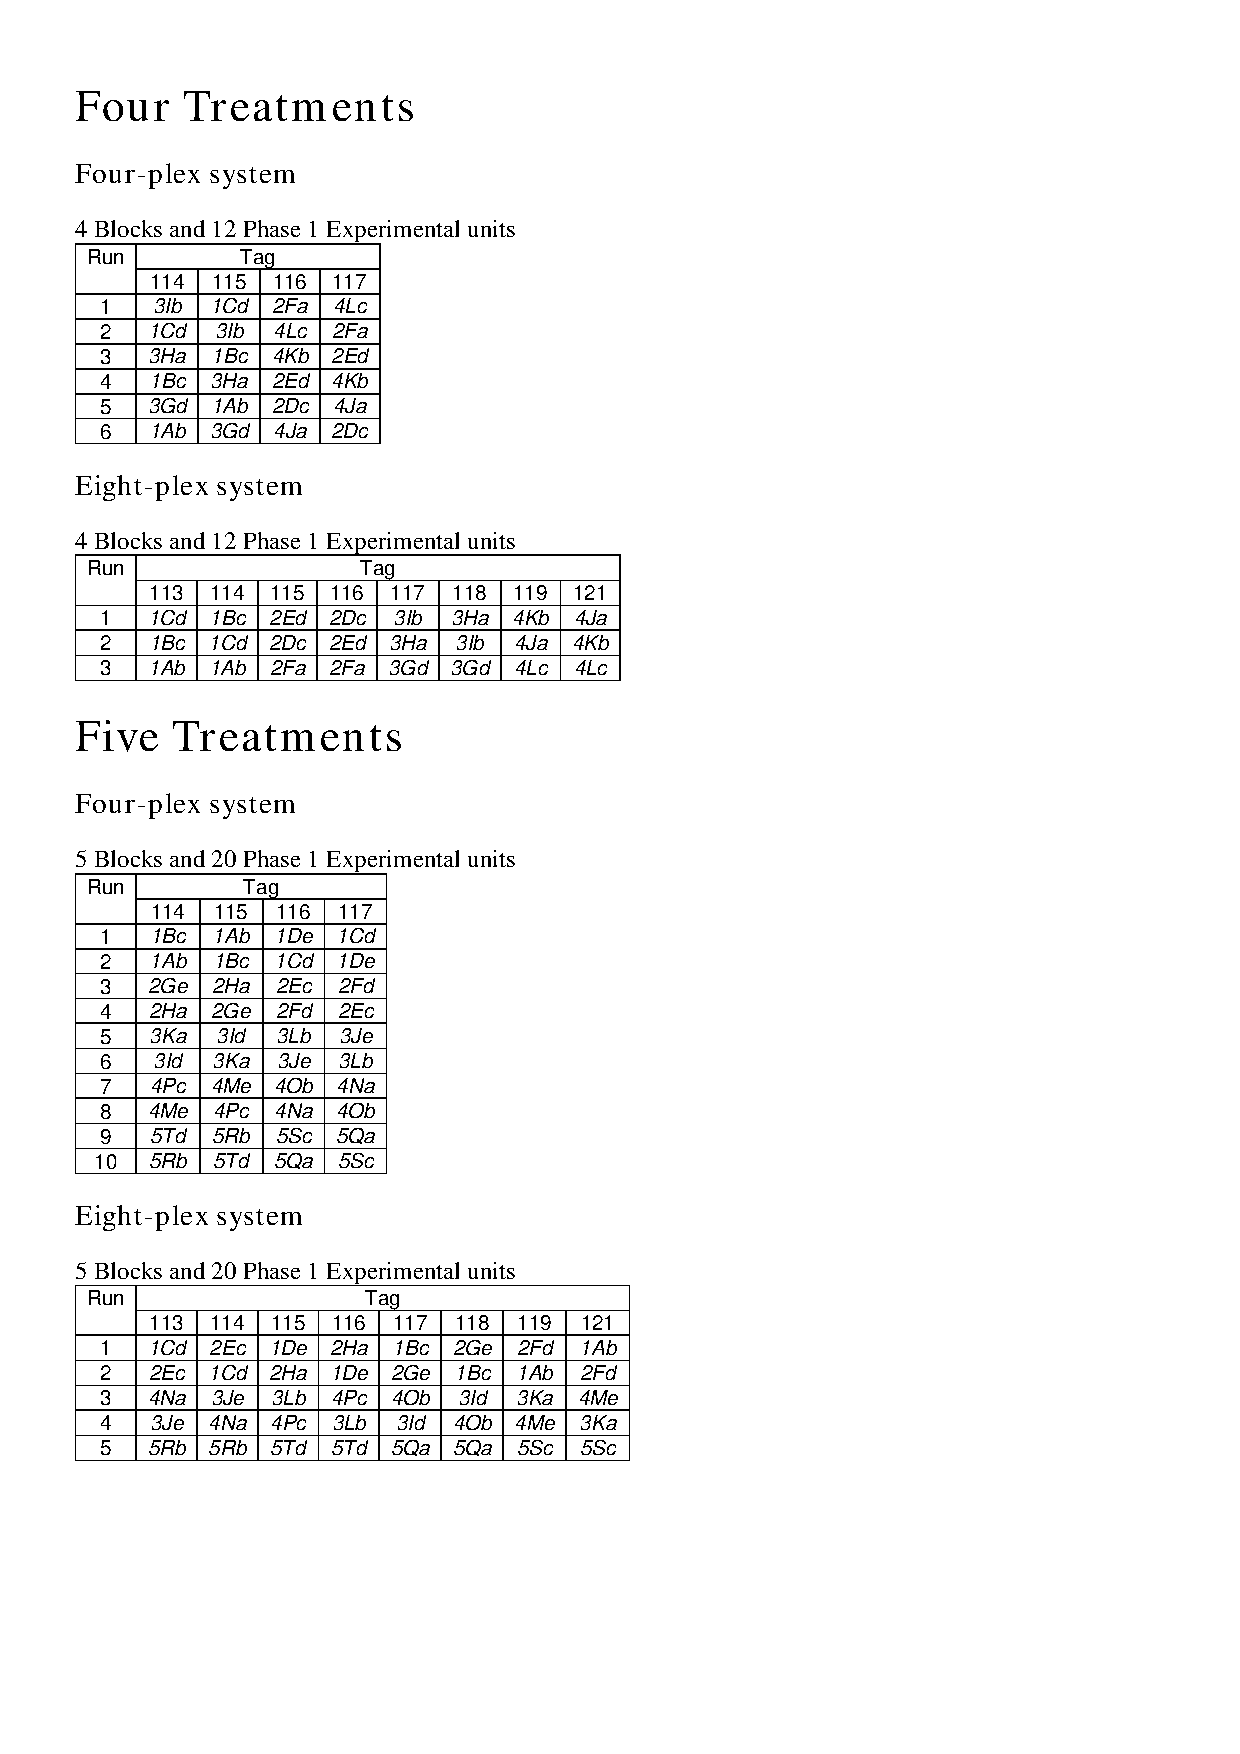
\includepdf[pages={1-},scale=1]{ChapterAppendix/BIBDdesigns.pdf}

\chapter{Tables of properties of optimal designs when Phase 1 is a BIBD} \label{append:optimalBIBD}

\includepdf[pages={1-},scale=1, fitpaper, rotateoversize]{ChapterAppendix/optimalBIBD.pdf}


